\documentclass[final-report.tex]{subfiles}

\begin{document}

\subsection{Literature Review}

Our systematic literature review (SLR) adhered to the methodological guidelines and procedural steps established by Gough et al. \cite{gough2017introduction} and Petticrew \& Roberts \cite{petticrew2008systematic}, which can be encapsulated as follows:
\begin{itemize}
    \item 1) Formulation of research questions and a conceptual framework; 
    \item 2) Searching and screening for pertinent literature based on predetermined eligibility criteria
    \item 3) Coding the literature to align with the conceptual framework
    \item 4) Employing quality appraisal criteria;
    \item 5) Synthesizing the selected studies within the context of the conceptual framework or using study codes;
    \item 6) Interpreting and disseminating the findings. 
\end{itemize}
These steps were executed in conjunction with the PRISMA guidelines provided by \cite{page2021prisma} to facilitate the various phases of the review process. 

\begin{figure}[!h]
    \begin{minipage}{0.4\textwidth}
        \centering
        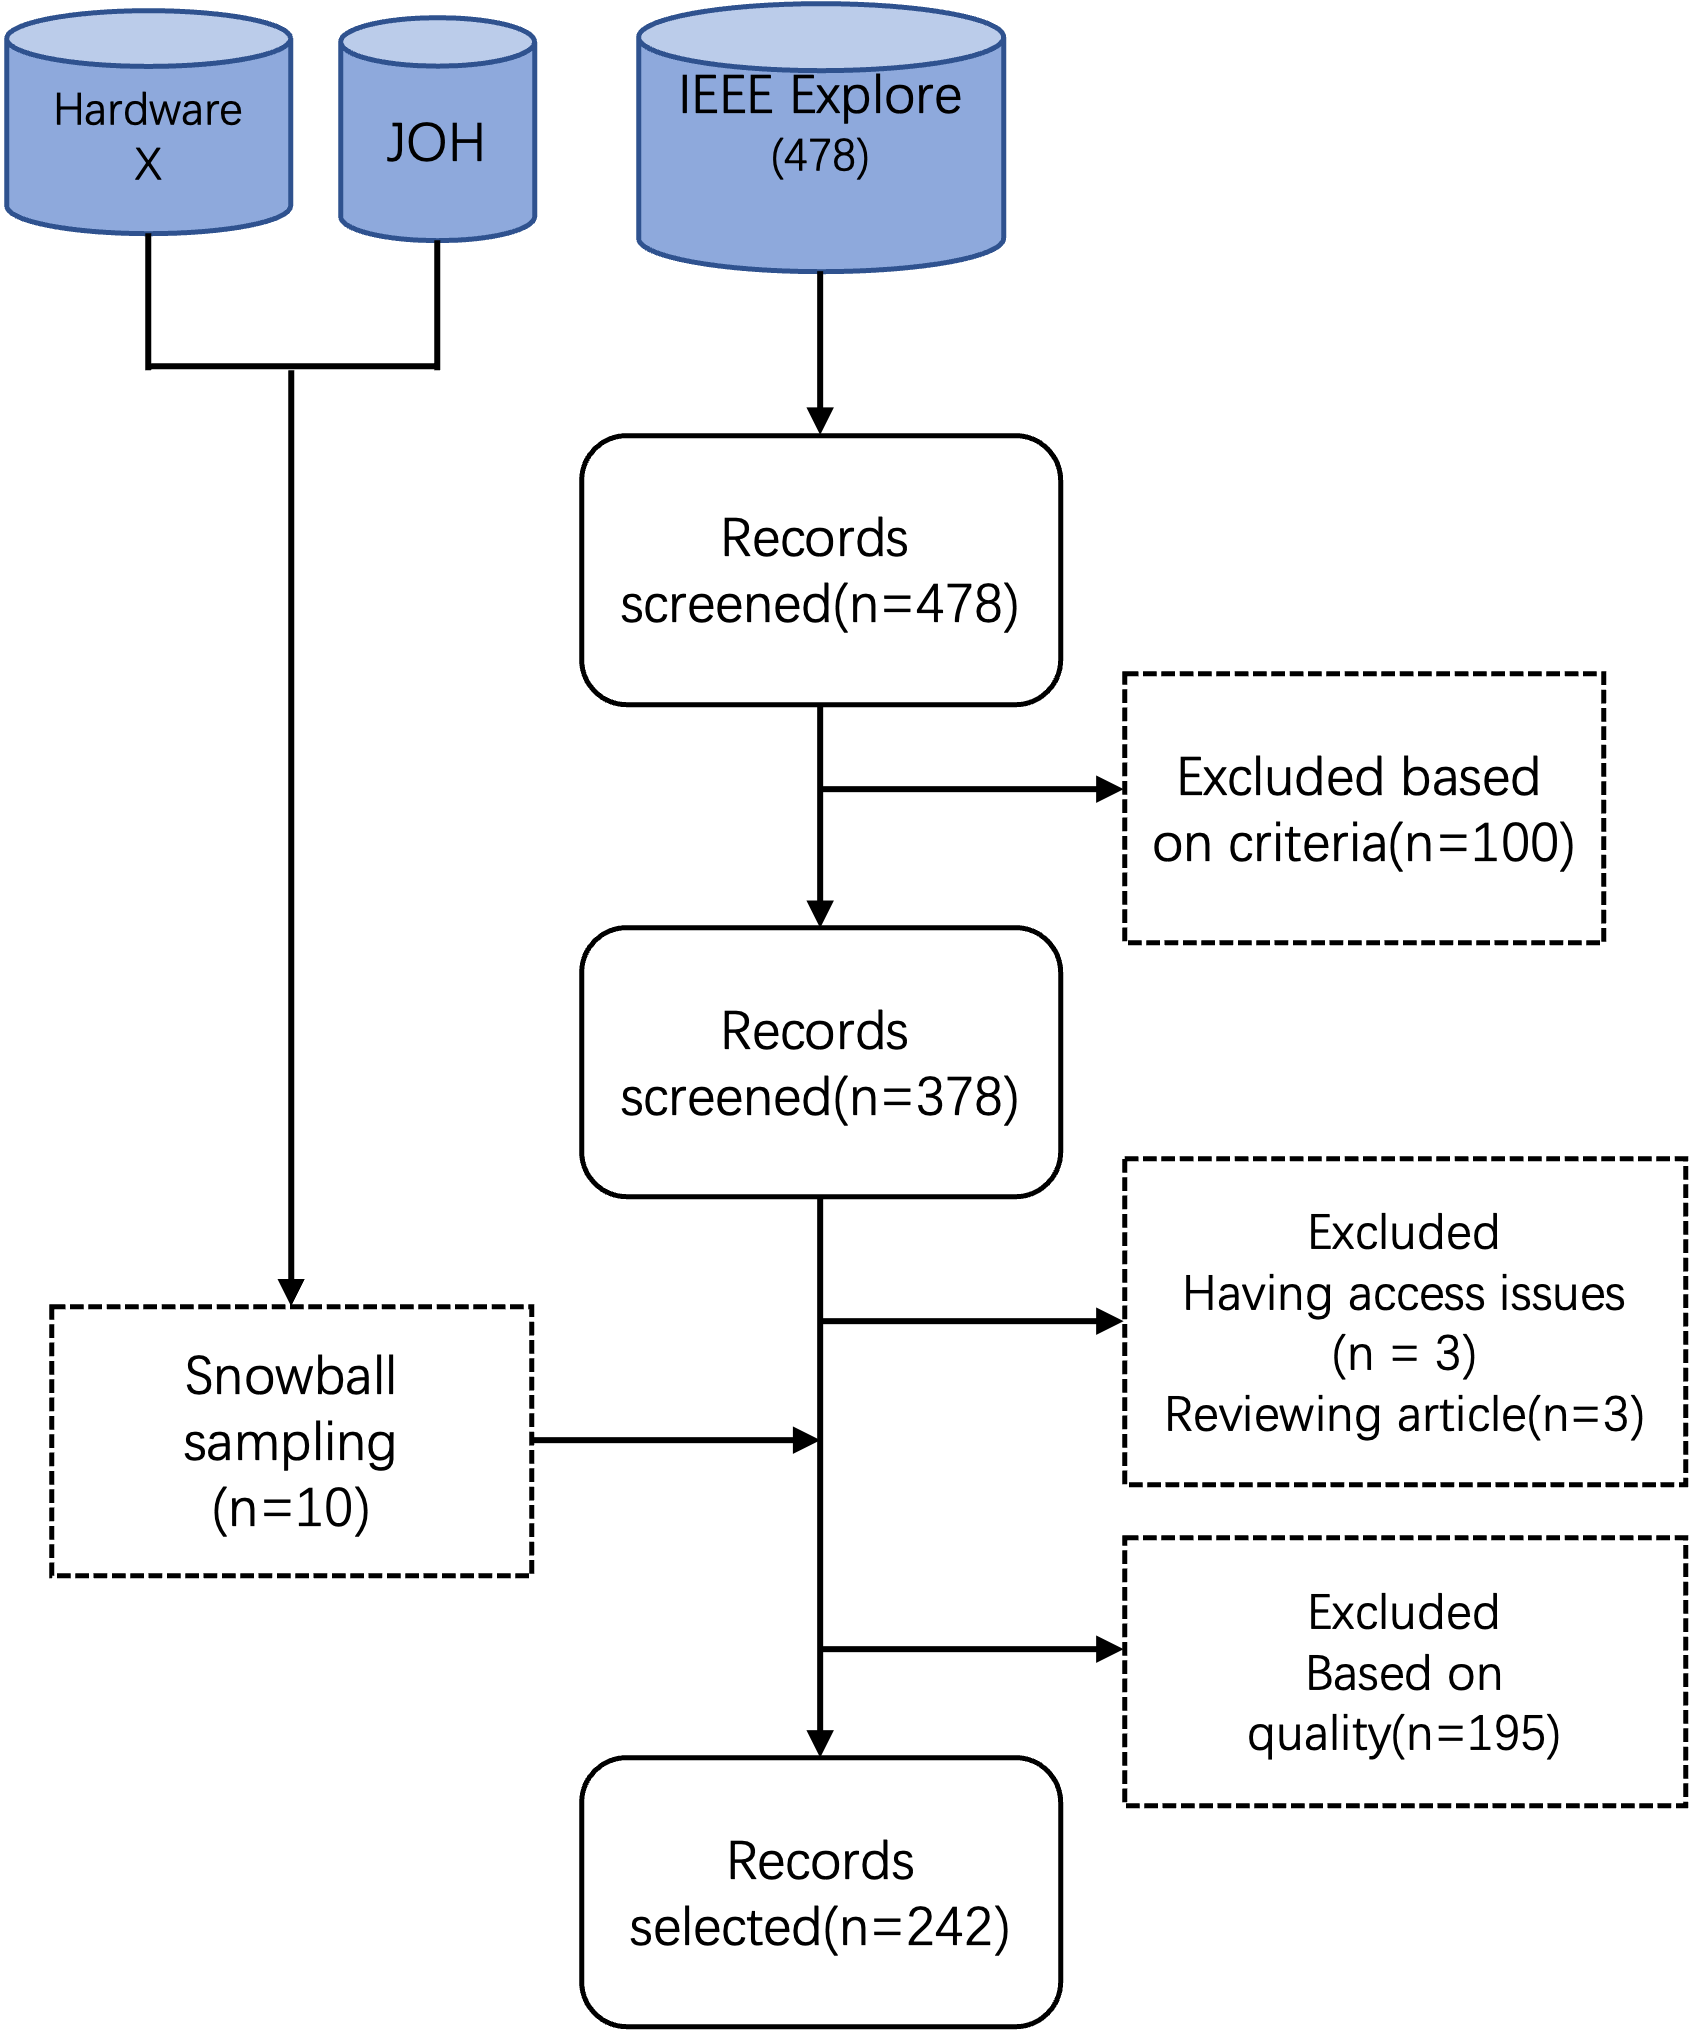
\includegraphics[width=\textwidth]{../Images/SLR.png}
        \caption{Systematic Literature Review Process}
        \label{fig:process}
    \end{minipage}
\end{figure}
Figure \ref{fig:process}
illustrates the stages of the SLR in accordance with the aforementioned guidelines.
To answer the question regarding the collaborative environments, our method is a grey literature review. 
The qualitative questions posed can be effectively answered by a systematic literature review, as the movement is very young. 
Most if not all the literature on the subject can be reviewed, along with all the projects listed by the Open Source Hardware Association.

% We started with a seed of papers on this subject, and we checked the citations used in the seeds recursively. 

% Part of the methodology would also be to read through all the literature in the two FOSH journals and to record summaries, benchmarks, and the licences of the hardware they proposed.
% These two journals are the 
% \begin{enumerate}
%     \item \href{https://openhardware.metajnl.com/}{Journal of Open Hardware}
%     \item \href{https://www.sciencedirect.com/journal/hardwarex}{HardwareX}
% \end{enumerate}

\subsubsection{Search Scope}

The publications of the FOSH journals were the initial pool of publications for our search. An effective strategy for acquiring a dependable collection of publications is to search through high-quality bibliographic databases \cite{petersen2015guidelines}. We chose databases that implement a discerning inclusion process, in which in-house editors assess prospective publication venues using factors such as the peer-review system, global diversity of editors and authors, citation influence, and self-citation rates. As a result, we identified the following databases, which have proven successful in prior secondary research: IEEE Explore, ACM library, and Scopus.

\subsubsection{Screening And Selection}
The search string underwent multiple refinements to maximize the number of relevant studies within the scope of the Systematic Literature Review (SLR). For example, the initial search string included terms such as "open-source hardware" and "open hardware," as demonstrated in block. 
\par
\begin{lstlisting}
("Document Title":open source hardware)
OR ("Document Title":opensource)
OR ("Document Title":open-source)
AND ("Abstract":hardware)
\end{lstlisting}
Subsequently, a secondary search string was constructed, incorporating key terms like "community," "state of the art," and "collaboration," which are commonly associated with FOSH applications used in academic and industrial research, as identified in systematic reviews.

This approach yielded a total of 372 records from the aforementioned sources. The records of the retrieved articles were exported to a CSV file to identify duplicates and complete any missing information.

The aforementioned query was executed on April 1st, 2023 and we defined the inclusion and exclusion criteria to filter the extracted publications from the databases. Specifically, the inclusion criteria were as follows:

\begin{table}[htbp]
\centering
\caption{Inclusion and Exclusion Criteria}
\begin{tabular}{|c|c|p{6.5cm}|}
\hline
\textbf{I/E} & \textbf{No.} & \multicolumn{1}{c|}{\textbf{Criteria}} \\
\hline
I & 1 & Include publications that addressed at least one of the research questions outlined in this study . \\
\hline
I & 2 & Include peer-reviewed primary studies that are relevant to FOSH (cross-checking and validation needed for such studies). \\
\hline
I & 3 & If there are multiple relevant studies that report the same research, then include the longest study only and exclude the rest of them. \\
\hline
E & 1 & Exclude publications not written in English \\
\hline
E & 2 & Exclude publications with no accessible full-text\\
\hline
E & 3 & Exclude tables of contents, editorials, white papers, commentaries, extended abstracts, communications, books, tutorials, non-peer-reviewed papers, and duplicates. \\
\hline
E & 4 & Exclude brief papers comprising fewer than six pages in single-column format. \\
\hline
E & 5 & Exclude review articles and secondary studies. \\
\hline
E & 6 & Exclude papers deemed irrelevant to FOSH based on title, abstract, keywords, introduction, and conclusion, requiring cross-checking and validation. \\
\hline
\end{tabular}
\label{tab:criteria}
\end{table}

In a distinct structure, the screening process for the n=478 records commenced with a review of the titles and abstracts. 
Studies that did not meet the inclusion criteria outlined in Table (3) and were not within the scope of the SLR were eliminated. 
Following this procedure, n=100 records from the IEEE explore database, as well as JOH and HardwareX journals, were excluded, leaving n=378 articles. 
The remaining articles were examined for eligibility, and those lacking a DOI, having access issues (n=3), or not being primary research (e.g., literature reviews and surveys) were removed (n=3). 
Subsequently, each remaining article was assessed based on a quality criterion employing a Likert scale survey, which ranged from 1 to 3, as shown in Table (2). 
These survey questions were designed with FOSH features and the SLR scope's relevance in mind. 
All questions carried equal weight, meaning that an article's overall score was determined by the average of these questions' scores. 
Ultimately, articles with a total average score above 12 were excluded, resulting in n=242 articles, as illustrated in Fig. (1).

\begin{table}[htbp]
\centering
\caption{Quality survey to assess the articles in the SLR.}
\begin{tabular}{|p{0.6\linewidth}|c|}
\hline
\textbf{Survey Questions} & \textbf{Range (1-3)} \\
\hline
Q1. Does the study describe clear criteria for the selection of the hardware used in the state of art senerio? & (1: agree to 3: disagree) \\
\hline
Q2. Does the study show a method and experiments that allow validating the state of art performance ? & (1: agree to 3: disagree) \\
\hline
Q3. Does the study mention the collaboration or other community related material of the FOSH? & (1: agree to 3: disagree) \\
\hline
Q4. Does the study indicate the scope and limitations of the FOSH developed? & (1: agree to 3: disagree) \\
\hline
Q5. Is the developed hardware application accessible, replicable, and reusable? & (1: agree to 3: disagree) \\
\hline
Q6. Has the study been cited by other authors? & (1: Yes, 3: No) \\
\hline
\end{tabular}
\end{table}


\subsubsection{Snowballing}

To expand the selection of investigations included in the SLR, snowballing guidelines provided by Wohlin \cite{wohlin2014guidelines} were utilized to ensure that our study did not overlook any pertinent publications. 
Upon filtering the initial sample set of publications, the snowballing method expanded the collection by examining their references as well. 
It is important to note that formal snowballing is an iterative process: during each cycle, new publications are identified, and their references are analyzed in subsequent iterations. 
However, due to the relatively small number of significant publications found in other sources, we conducted only one iteration, resulting in the addition of n=10 publications from sources beyond the primary database, IEEE. 
Notably, specialized OSHW journals, such as HardwareX and Journal of Open Hardware (JOH), were incorporated into the search process.

\subsubsection{Data Extraction and Analysis}
During the data extraction and analysis phase, we employed a clustering technique to categorize the documents based on their textual content. 
Specifically, we applied the K-means clustering algorithm to group the articles according to the similarity of their titles and abstracts within the TF-IDF feature space, which is a numerical representation of the importance of words in the documents.

To ascertain the optimal number of clusters (k), we examined the elbow method and silhouette scores, which offer insights into the ideal cluster count by taking into account the within-cluster sum of squares and the average silhouette width, respectively. 
After determining the optimal k value, we implemented the K-means clustering algorithm and allocated each document to its corresponding cluster.

For a better interpretation of the results and a deeper understanding of the themes or topics within each cluster, we extracted the top keywords associated with each cluster. 
Furthermore, we generated word clouds to visually represent the most prominent keywords within each cluster, which facilitated the identification of prevalent themes and topics. 
This approach provided valuable insights into the connections between the articles and their potential relevance to the research objectives, while also offering an accessible and engaging means of conveying the information.

\subsection{Scripts And API}

The 
\href{https://www.oshwa.org/}{Open Source Hardware Association} 
tracks all FOSH projects. 
It also provides an 
\href{https://certificationapi.oshwa.org/documentation}{API}
that can be used to query information on licensing and collaboration environments.

We used this API to collect all FOSH projects tracked to date.
These projects have three pieces with licences; these are hardware, software, and documentation. 
Additionally, the API was used to collect the websites, and platforms used to store the project. 
Mostly these platforms are GitHub, and as such the number of forks, comments, issues, contributors are also scraped using the GitHub API. 


\subsection{Limitations}

Despite the application of rigorous protocols for data collection and analysis throughout the systematic literature review, certain limitations were encountered. 
One of these limitations pertains to the selection of databases used in the search process. 
The chosen database was selected due to its extensive collection of FOSH-related studies and its ability to provide a substantial corpus of designs for analysis under the PRISMA guidelines. 
Nevertheless, future studies could benefit from including more comprehensive databases such as Scopus, Web of Science(WoS), ACM Guide to Computing Literature, and Google Scholar to further supplement and expand upon the findings of this research.

Second limitation of this study arises from the selected timeframe (2017-2022). 
This period was chosen because it encompasses a substantial portion of the relevant designs and aligns with the state-of-the-art FOSH technologies, such as NVidia Jetson, Arduino, Raspberry Pi. 
However, it is important to acknowledge that some significant studies may fall outside of this timeframe or may have garnered citations after the search date, potentially impacting the comprehensiveness of the review.

A third limitation pertains to the search strings. 
Standardized terms, such as "open-source hardware," were employed; however, this may have led to the exclusion of other terms or more specific terminology (e.g., collaboration hardware, open innovation) that researchers use to describe their developments or target audiences in the SLR process.
Limitation can also stem from the exclusion of gray literature, such as white papers, preprints, or working papers, as well as documents not written in English. 
This constraint is inherent in the features and procedures of an SLR, limiting the range of document sources that researchers can analyze and potentially affecting the comprehensiveness of the findings.

A fourth limitation arises from the time constraints associated with this project. 
Although our initial plan was to search all available databases for FOSH, our results primarily came from the IEEE database. 
We conjecture that platforms such as GitHub repositories may also host state-of-the-art open-source hardware projects, but due to time restrictions, we were unable to include them in our search. 
This limitation may impact the comprehensiveness and generalizability of our findings.

A fifth limitation pertains to the data analysis phase. 
Although we employed a clustering technique, more advanced professional tools could have been utilized for a comprehensive bibliometric analysis. 
Examples of such tools include, VOSViewer \cite{van2013vosviewer}, and Crossref REST API \cite{lammey2016using}, which are designed for network data analysis, focusing on items and clusters while providing overall functions to create and visualize maps. 
Some text analytics tool like Leximancer \cite{sotiriadou2014choosing} that can analyze the contents of document collections and visualize their trends in concept maps. 
The use of these advanced tools might have yielded additional insights and a more in-depth understanding of the relationships and patterns within the data.

Additionally, the use of the K-means clustering algorithm in our data analysis phase has its inherent limitations. 
K-means clustering assumes that the clusters are spherical and equally sized, which might not always be the case for real-world datasets. 
Moreover, it is sensitive to the initial placement of cluster centroids and may converge to a local optimum. 
While we made efforts to determine the optimal number of clusters using methods like the elbow method and silhouette scores, alternative clustering algorithms, such as hierarchical clustering or DBSCAN, could potentially provide different perspectives on the structure of the data.

\end{document}
